\section{Data Fidelity}
\label{sec-fidelity}

The final and most important measure of our network is its ability to
provide scientifically-meaningful data on the volcano's activity. In
this section, we perform an initial analysis of the seismic and
acoustic signals from a seismological perspective, with the goal of
validating the accuracy of the signal quality and timing.

\subsection{Acoustic wave propagation}
%  - Arrival time distribution across the array [KL]
%    - Back-projection to possible event sources
%    - Consistency with Reftek data

The infrasonic (low-frequency acoustic) waves generated by the
volcano are primarily the result of explosive events. 
%% As such, infrasound is a useful complement to seismic monitoring and
%% can be used to differentiate explosions from other kinds of
%% earthquakes.
We start by measuring the velocity of infrasonic waves recorded by our
network, which is more straightforward than seismic analysis for
several reasons.  First, infrasonic waves generate a clear
impulse in the microphone signal, making it easy to determine the
time of the wave arrival at each sensor. In addition, acoustic waves
propagate about an order of magnitude slower than seismic waves
(roughly 340~m/s versus 1500-4000~m/s).
%% , and compared to ground-propagating seismic waves, air is a
%% relatively homogenous medium.
We also expect an infrasonic wave to originate at the 
vent of the volcano, simplifying the wave velocity calculation.

%% \begin{figure*}[t]
%% \begin{center}
%% \begin{tabular}{cc}
%% 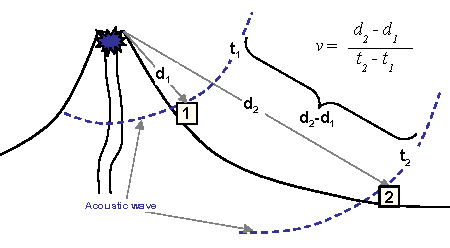
\includegraphics[width=0.4\hsize]{./evaluation/figs/fidelity/acousticSeismicSketches.pdf}
%% &
%% 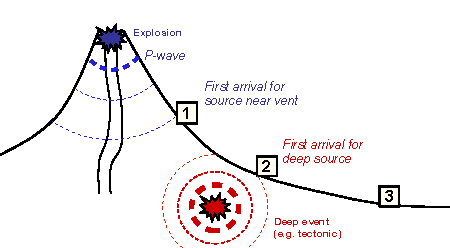
\includegraphics[width=0.4\hsize]{./evaluation/figs/fidelity/acousticSeismicSketches2.pdf}
%% \\
%% {\small\bf (a) Acoustic wave propagation} &
%% {\small\bf (b) Seismic wave propagation} \\
%% \end{tabular}
%% \end{center} 
%% \caption{\small {\bf Computing wave arrivals of seismic and acoustic
%% waves.} {\em These sketches show the propagation of (a) acoustic
%% and (b) seismic waves from the volcano. While acoustic waves emanate
%% from the vent, seismic waves may be generated by explosions from the
%% vent or sources within the volcano.}}
%% \label{fig-acousticSketch}
%% \label{fig-seismicSketch}
%% \end{figure*}

\begin{figure}[t]
\begin{center}
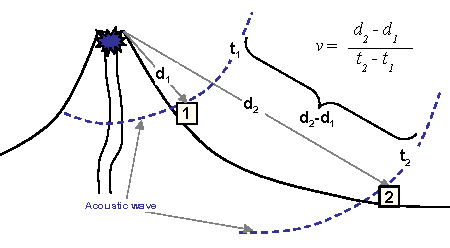
\includegraphics[width=\hsize]{./evaluation/figs/fidelity/acousticSeismicSketches.pdf}
\end{center}
\caption{\small{\bf Computing acoustic wave velocity.}  
{\em The velocity of the acoustic wave is calculated based on
the distance of each station from the vent, $d_i$, and the 
arrival time of the wave at each station, $t_i$.}}
\label{fig-acousticSketch}
\end{figure}

We identified four events in our data set with a clear infrasonic
component. For each event, we hand-picked the arrival time of the wave
at each node using the time-rectified signal.
Figure~\ref{fig-acousticArrival} plots the wave arrival time versus
the distance of each node from the vent. As shown in
Figure~\ref{fig-acousticSketch}, the velocity of the wave can be 
calculated by performing a linear regression on this dataset.

\begin{figure}[t]
\begin{center}
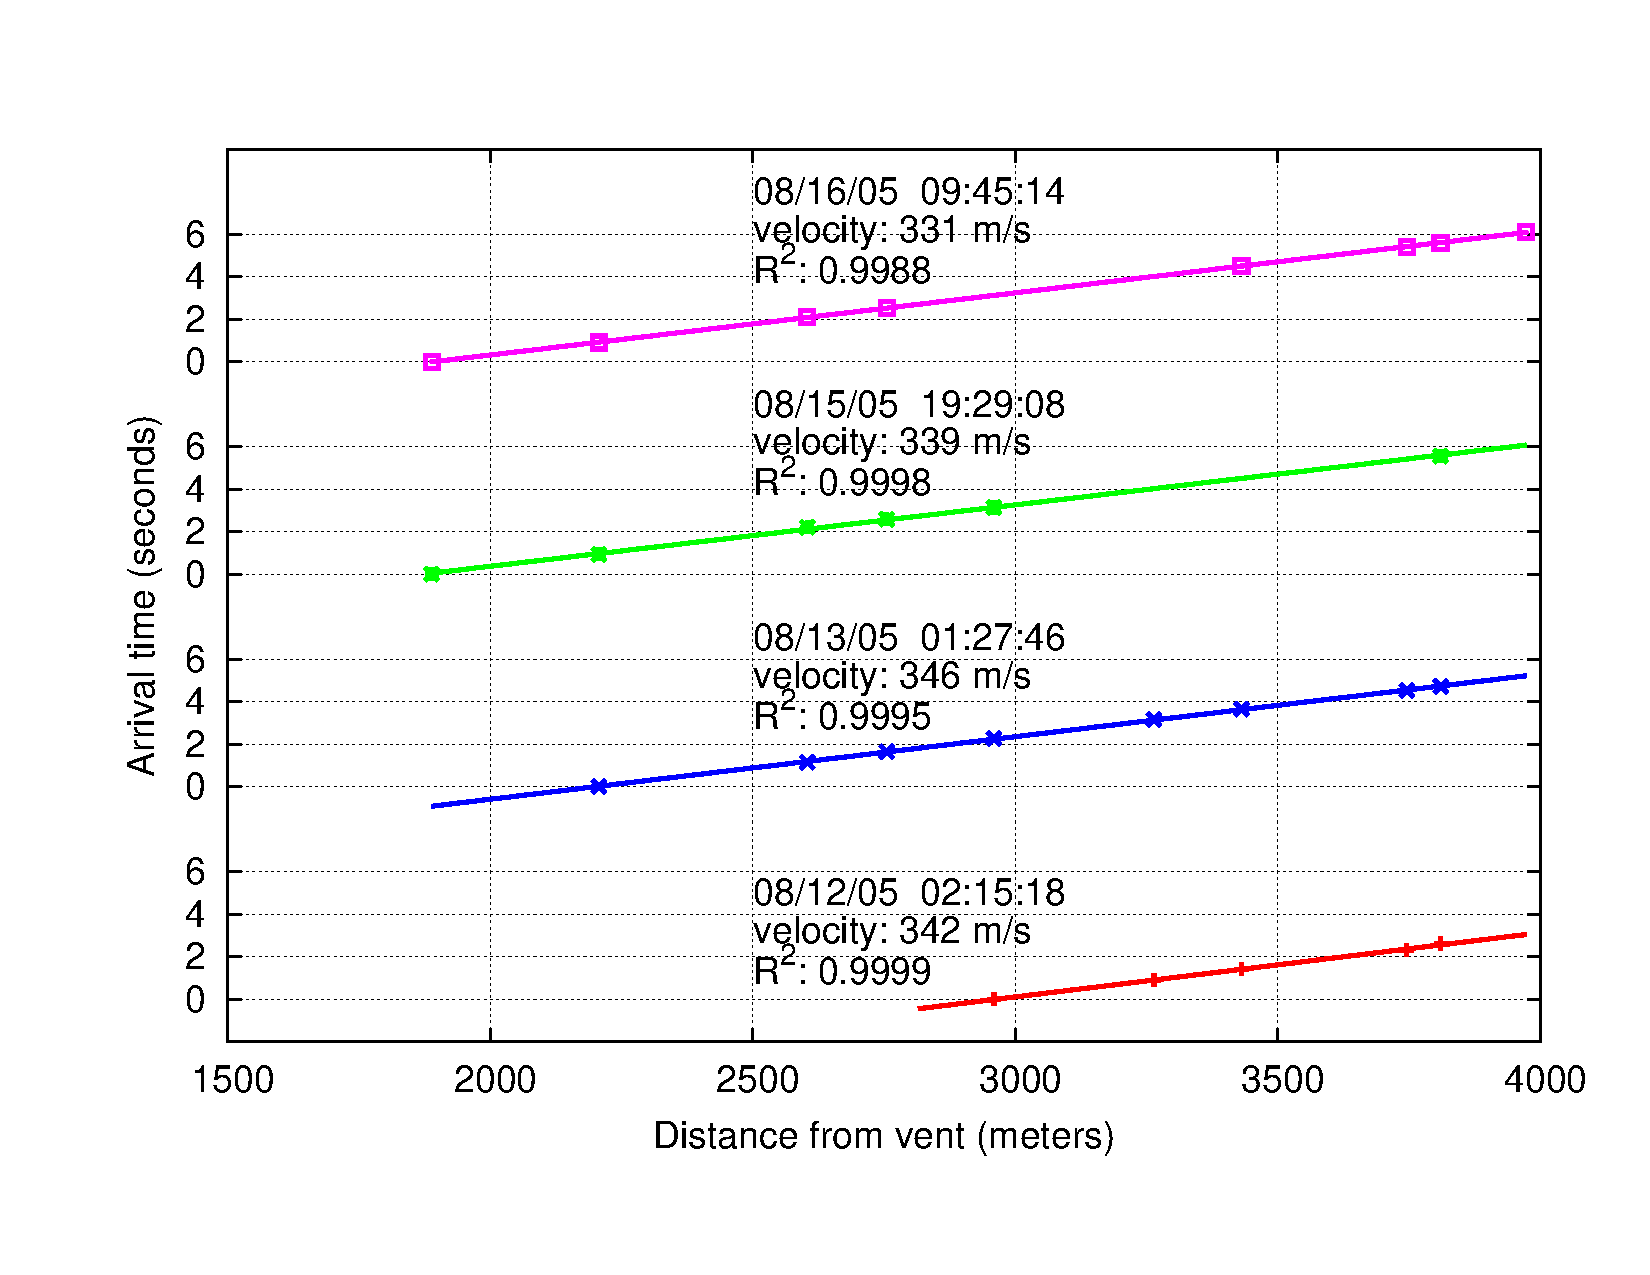
\includegraphics[width=\hsize]{./evaluation/figs/fidelity/acousticArrival/acoustic.pdf}
\end{center}
\caption{\small{\bf Acoustic wave arrival times and velocity.}
{\em This figure shows the acoustic wave arrival time vs. distance
from the vent for 4~separate events. Also shown is the resulting
acoustic wave velocity and the $R^2$ coefficient of determination.}}
\label{fig-acousticArrival}
\end{figure}

The result of this calculation is also shown in
Figure~\ref{fig-acousticArrival}.  The velocity of sound in air is
temperature-dependent; for temperatures between 10--20 $^{\circ}$C
the velocity range is 337--343~m/s.  The calculated wave velocities are
mostly in this range, with a mean of 339.5~m/s. The coefficients of
determination $R^2$ are very high, between
0.9988~and~0.9999, showing that the timing and quality of the
acoustic data closely matches our expectation
of the infrasonic waves produced by the volcano.

%\begin{figure}[t]
%  \begin{small}
%    \begin{center}
%      \begin{tabular}{|ccc|} \hline
%               {\bf Event} & {\bf Velocity m/s)} & {\bf $R^2$} \\ \hline
%               08/12/05 02:15:18 & 331 & 0.9988 \\
%               08/13/05 01:27:46 & 339 & 0.9998 \\
%               08/15/05 19:29:08 & 346 & 0.9995 \\
%               08/16/05 09:45:14 & 342 & 0.9999 \\ \hline
%               {\bf Mean} & 339.5 & 0.9995 \\
%               {\bf StdDev} & 6.35 & 0.0005 \\ \hline
%      \end{tabular}
%    \end{center}
%  \end{small}
%  \caption{\small{\bf Acoustic time of arrival summary.}  {\em This
%          table summarizes the acoustic wave velocity and $R^2$ from
%          our linear regression.  The mean velocity for the 4 events
%          is 339.5~$m/s$ which is between the expected velocity of
%          soundm, 337~$m/s$ at 10\textcelsius $ $ and 343~$m/s$ at
%          20\textcelsius. The $R^2$ coefficient is very close to 1.0,
%          indicating a very strong correlation.}}
%  \label{fig-acousticArrivalReg}
%\end{figure}

\subsection{Seismic wave propagation}
%% - How different from acoustic data
%% - Do our analysis in two parts
%%   - data consistency across a larger number of events.  Here we
%%     want to asses that our data meets certain conditions
%%   - detailed analysis on a XXX events (JJ's section)

Analyzing the seismic waves captured by our network is
significantly more challenging. This is primarily because the 
source locations of seismic waves are unknown. 
Seismic events may originate at the vent (in the case of an explosion)
or deep within the edifice, producing very different patterns of
P-~and S-wave arrivals at each node. A full seismological analysis
of our data is beyond the scope of this paper. However, we 
present a high-level measure of the {\em consistency} of the 
signals captured by our network: that is, we evaluate whether
the seismic wave arrivals are consistent with expected volcanic
activity.

%% Our sensor array was established in a radial geometry for two primary
%% reasons: (1) to understand the attenuation structure of volcanic
%% explosion earthquakes, and (2) to calculate the seismic wavefield
%% incidence for events occurring near the volcanic conduit. Seismic
%% wavefield incidence is an especially important parameter to recover
%% because it provides us with information about the relative depth of
%% volcanic earthquakes. In addition, knowing the velocity structure of the volcanic edifice 
%% provides important geophysical constraints that are used to assess
%% earthquake source parameters.

%% Our sensor array was established in a radial geometry for two 
%% primary reasons: (1) to understand the attenuation structure of 
%% volcanic explosion earthquakes, and (2) to calculate the seismic 
%% wavefield incidence for events occurring near the volcanic
%% conduit.  
%% %Both seismic attenuation, which is the study of how seismic
%% %ground shaking decreases with propagation distance and frequency
%% %content, and wavefield analyses are the focus of ongoing study with
%% %the collected dataset.
%% Seismic wavefield incidence is an especially important parameter to
%% recover because it provides us with information about the relative
%% depth of volcanic earthquakes.  
%For a simplified 2-D geometry, the apparent velocity $V_a$ of seismic
%wave arrivals across the array is determined by the intrinsic 
%P-wave velocity $V_p$ of the medium and angle of incidence $\theta$ 
%of seismic energy on the array: $V_a = V_p / \cos(\theta)$.  
%Typically depth is hard
%to determine through traditional means because seismic stations at
%volcanoes are most easily deployed around the periphery of the volcano
%(providing good epicentral locations but poor depth constraints).  
%
%Our sensors were deployed along a radial trajectory away
%from the vent in order to calculate the move-out of first arrivals
%(i.e., time distribution of compressional P-Wave first arrivals).
%This allows us to discriminate sources originating in the shallow
%portion of the cone near the vent from events occurring more deeply.
%Furthermore, variations in apparent velocity, calculated from the
%move-out, enable us to estimate origin depth of various events.
%
%For a near-surface source in the vicinity of the
%vent, $\theta$ approaches zero and apparent velocity approaches intrinsic
%compressional velocity of the medium.  Conversely, for a deeper source
%(i.e., volcano-tectonic event), seismic angles can steeply impinge
%upon the free surface of the volcanic edifice leading to infinite
%apparent velocity.  For both types of events presented in Figure 3, the
%lowest apparent velocities (1.5 to 2.0 km/s) is observed towards the
%far end of the array (Figure 3).  This is the value that most closely
%approximates the seismic P-wave velocity of the volcano in this locale.
%% In addition, knowing the velocity structure of the volcanic edifice 
%% provides important geophysical constraints that are used to assess earthquake
%% source parameters.

\begin{figure}[t]
\begin{center}
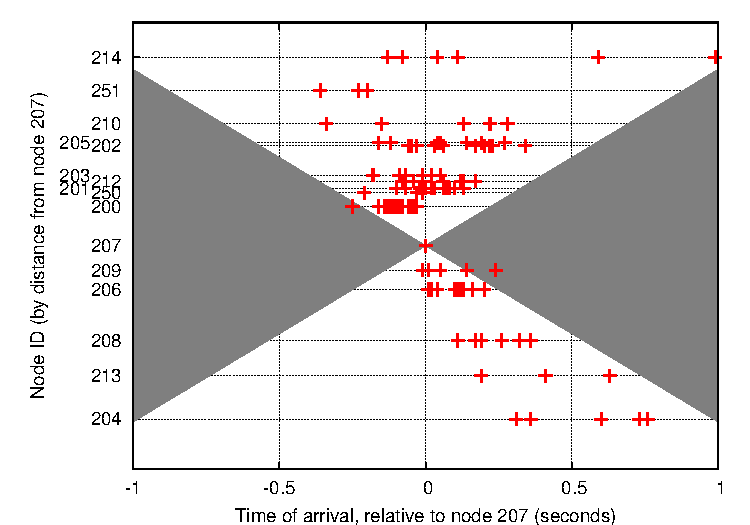
\includegraphics[width=\hsize]{./evaluation/figs/fidelity/seismicArrival/arrivalTimesPlotScatteredNode.pdf}
\end{center}
\caption{\small{\bf Time of arrival of each node over multiple
events.}  {\em This graph shows the spread of arrival times for each
node.  The arrival time and distance is relative to node~207.  The
arrival time for each node is fairly consistent over multiple events,
with the exception of node~214.  The shaded area indicates a move-out
velocity of less than 1,500 $m/s$.}}
\label{fig-seismicArrivalScatteredNode}
\end{figure}

The most natural measure of data consistency is whether the
time of the seismic P-wave arrival at each sensor falls within 
an expected {\em envelope} based on the minimum speed at which
seismic waves are believed to propagate at Reventador, which 
we estimate as 1500~m/s. We took 15~seismic events with clear
P-wave arrivals and used an automatic algorithm~\cite{pwave-picking} to 
determine the wave arrival time.\footnote{Unlike acoustic
waves, determining seismic wave arrival times is notoriously 
difficult. The seismograms in Figures~\ref{fig-jjExplosion}
and Figure~\ref{fig-jjTectonic} should give the reader some
appreciation for this.} 

Figure~\ref{fig-seismicArrivalScatteredNode} shows a scatterplot of
the arrival times with respect to node~207, which was chosen as an
arbitrary reference point since data for this node appeared in all
15~events. The $y$-axis represents the distance of each node
from~207. Depending on the seismic source location, we expect waves to
arrive both before and after node~207.  However, the slowest wave
speed (1500~m/s) dictates the maximum difference in the wave arrival
between each station.\footnote{Note that there is no lower bound on
arrival times, since a wave emanating from a deep source could arrive
at all stations nearly simultaneously.} The shaded area in
Figure~\ref{fig-seismicArrivalScatteredNode} covers the ``exclusion
envelope'' of arrival times at each station.  As the figure shows,
only 2~out of~124 arrivals fall outside of this envelope.

%It is interesting to note that although node~204 is closest
%to the vent, seismic waves do not appear to reach this node first;
%this suggests a deep source under the middle of the sensor array,
%which is by itself an interesting scientific finding.

%The automated picking algorithm uses a tiered approach.  Seismograms
%are initially prepared by extracting the envelope waveform using the
%Hilbert transform.  This is followed by a median smoothing filter to
%remove noise glitches and otherwise undesirable high frequency
%signals.  The smoothed envelopes are then passed through a series of
%gradually refined forward-backward (sometimes called STA/LTA)
%root-mean-square ratio estimate.  Arrival times where significant
%changes in the ratio curves occur are saved.  Several thresholds are
%examined statistically and the initial estimate of the pick is
%determined by robust quantile cut-offs.
%
%This initial arrival time estimate is then used as a first guess
%provided to the so-called ARAIC algorithm (Auto-Regressive Akaiki
%Information Criterion) of Sleeman and van Eck~\cite{pwave-picking}.
%The ARAIC method uses an autoregressive characterization of the noise
%and signal and finds the time along the trace that minimizes the
%maximum likelihood function fit to the AR models.  The algorithms were
%implemented in R~\cite{r-book}, an interactive computation platform.

\begin{figure}[t]
\begin{center}
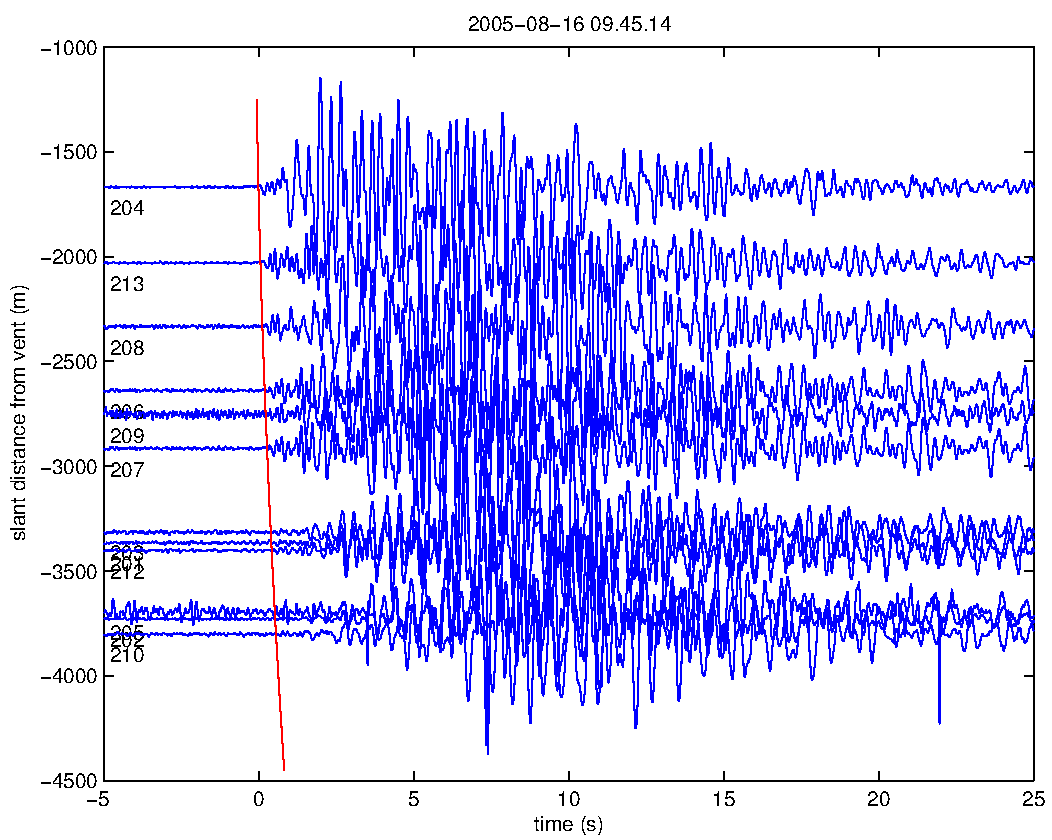
\includegraphics[width=\hsize]{./evaluation/figs/fidelity/seismicArrival/johnson/2005-08-16_09-45-14.pdf}
\end{center}
\caption{\small{\bf Explosion earthquake event at 08/16/2005 09:45:14 GMT.}
{\em P-wave arrivals have been identified manually and a second-order
polynomial (solid line) is fit to the arrivals. The arrival time
move-outs are consistent with a shallow near-vent source.}}
\label{fig-jjExplosion}
\end{figure}


Finally, we take a closer look at two seismic events recorded by our
array.  Figures~\ref{fig-jjExplosion}~and~\ref{fig-jjTectonic} show
seismograms from each of the sensor nodes after time rectification.
The $y$-axis corresponds to the distance of each node from the vent.
For each event, the P-wave arrivals have been determined by hand and a
second-order polynomial has been fit to the arrival times at each node
for clarity.

These two events show a very different pattern of wave arrival
times. Figure~\ref{fig-jjExplosion} shows the seismic wave
arriving first at stations near the vent (nodes~204 and 213). This
is consistent with a shallow near-vent source corresponding to an
explosion. This is confirmed by the corresponding acoustic data (shown
in Figure~\ref{fig-acousticArrival}) attributed to explosive expansion
of gas. 

In contrast, Figure~\ref{fig-jjTectonic} shows an event with the earliest
arrivals in the middle of the sensor array and the endpoints relatively
delayed; many such events were recorded by our network. 
This distribution implies a deeper source.  At the same time,
seismic velocity in the uppermost cone, which is comprised of unconsolidated
volcanic deposits, is presumed to be slower.  Such volcano-tectonic events
are likely generated by the fracturing of solid media typically induced
by pressurization within the edifice. This preliminary study
demonstrates the value of our wireless sensor network for collecting
accurate signals that can be subjected to seismological analysis.

\begin{figure}[t]
\begin{center}
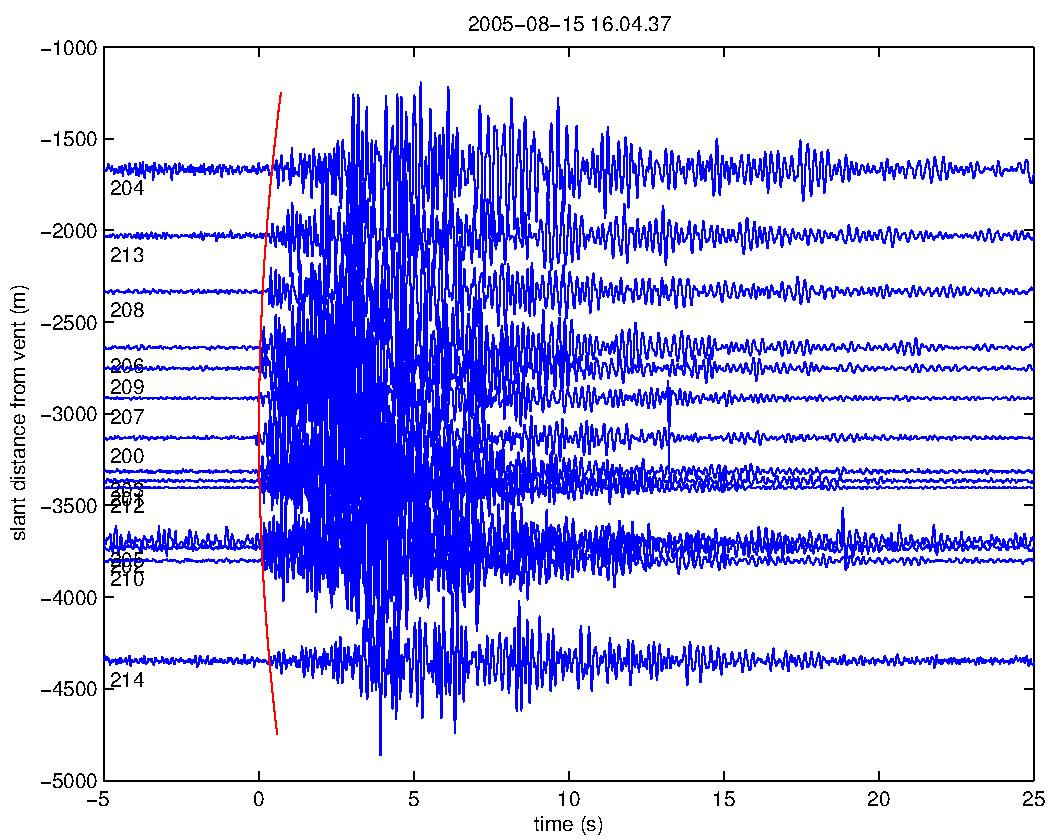
\includegraphics[width=\hsize]{./evaluation/figs/fidelity/seismicArrival/johnson/2005-08-15_16-04-37.pdf}
\end{center}
\caption{\small{\bf Tectonic earthquake event at 08/15/2005 16:04:37
GMT.} {\em In this event, seismic waves are first recorded near the
middle of the sensor array. This is due either to a source closer 
to the center of the array, variations in velocity structure, 
or most likely both.}}
\label{fig-jjTectonic}
\end{figure}


%%%%%%%%%%%%% OLD text %%%%%%%%%%%%%%%%%%%%%%%%
% - How different from acoustic
% - Subset of events that we analyzed
% - How we did linear fit and table fo results

%% \begin{figure}[t]
%% \begin{center}
%% 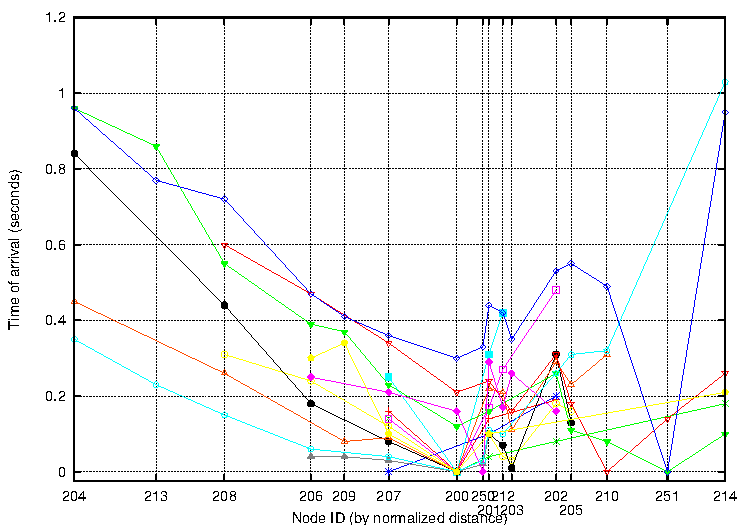
\includegraphics[width=\hsize]{./evaluation/figs/fidelity/seismicArrival/arrivalTimesPlot.pdf}
%% \end{center}
%% \caption{\small{\bf Time of arrival for the seismic data.}
%% {\em This figure shows the seismic wave arrival time offset by the
%% first arrival vs. normalized distance between nodes.  The graph indicates that
%% most events originate closer to the center of the array.}}
%% \label{fig-seismicArrival}
%% \end{figure}

%% \begin{figure}[t]
%% \begin{center}
%% 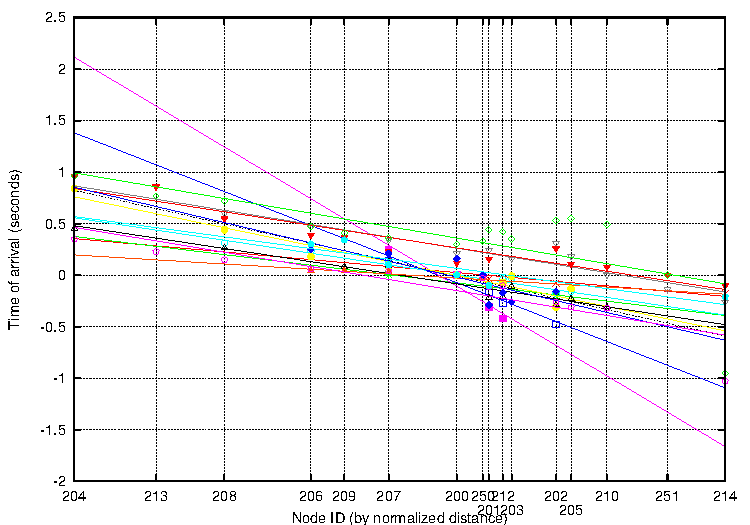
\includegraphics[width=\hsize]{./evaluation/figs/fidelity/seismicArrival/arrivalTimesPlotFit.pdf}
%% \end{center}
%% \caption{\small{\bf Liner regression for the time of arrival for the seismic data.}
%% {\em This arrival times of nodes to the right of the node with
%% the first arrival are mirrored about the x-axis.  This allows us to
%% draw a linear fit through the data points.  As we can see, most events
%% have a similar slope which indicates consistent wave velocities.}}
%% \label{fig-seismicArrivalFit}
%% \end{figure}

%% \begin{figure}[t]
%% \begin{center}
%% 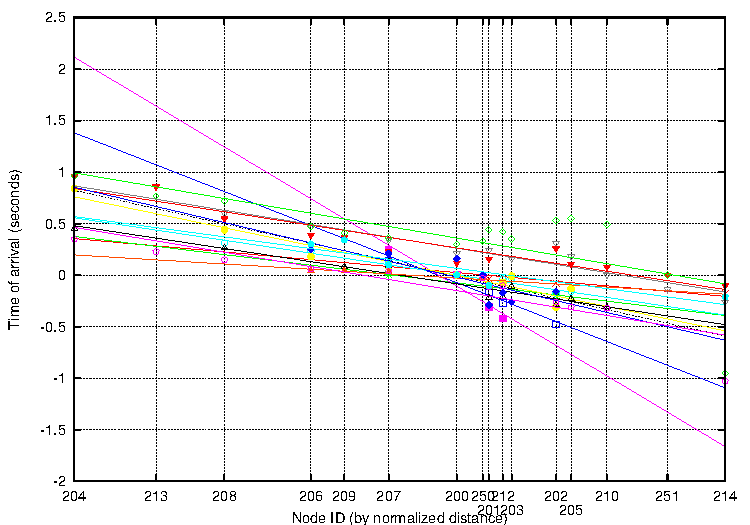
\includegraphics[width=\hsize]{./evaluation/figs/fidelity/seismicArrival/arrivalTimesPlotFit.pdf}
%% \end{center}
%% \caption{\small{\bf Liner regression for the time of arrival for the seismic data.}
%% {\em This arrival times of nodes to the right of the node with
%% the first arrival are mirrored about the x-axis.  This allows us to
%% draw a linear fit through the data points.  As we can see, most events
%% have a similar slope which indicates consistent wave velocities.}}
%% \label{fig-seismicArrivalFit}
%% \end{figure}

%% \begin{figure}[t]
%% %  \begin{minipage}[t]{.45\textwidth}
%%   \begin{small}
%%     \begin{center}
%%       \begin{tabular}{|ccc|} \hline
%%                {\bf Event} & {\bf Velocity (m/s)} & {\bf $R^2$} \\ \hline
%%                2005-08-11\_08.33.49 & 2356.97 & 0.91 \\
%%                2005-08-11\_09.12.38 & 5519.13 & 0.89 \\
%%                2005-08-11\_15.04.27 & 4287.73 & 0.99 \\
%%                2005-08-12\_00.30.40 & 1324.12 & 0.96 \\
%%                2005-08-12\_02.15.18 &  832.95 & 0.93 \\
%%                2005-08-13\_02.17.32 & 3376.40 & 0.96 \\
%%                2005-08-13\_04.24.42 & 2406.30 & 0.94 \\
%%                2005-08-13\_07.08.05 & 3241.98 & 0.95 \\
%%                2005-08-14\_04.32.29 & 8204.96 & 0.67 \\
%%                2005-08-14\_20.17.02 & 3061.23 & 0.87 \\
%%                2005-08-15\_09.11.28 & 3175.71 & 0.89 \\
%%                2005-08-15\_16.04.37 & 2903.11 & 0.51 \\
%%                2005-08-16\_01.32.19 & 2173.40 & 0.65 \\
%%                2005-08-16\_18.30.04 & 2981.71 & 0.77 \\
%%                2005-08-18\_02.45.51 & 3621.04 & 0.81 \\ \hline
%%       \end{tabular}
%%     \end{center}
%%   \end{small}
%%   \caption{\small{\bf Coefficient of determination ($R^{2}$) for events.}
%%           {\em The coefficien of determination is a measure of how well the
%%           regression line represents the data.  A coefficient value greater than
%%           0.65 is generally described as a strong correlation.  As we can see,
%%           most of our events have a coorelation higher than 0.65 indicating a good fit.}}
%%   \label{fig-seismicArrivalReg}
%% %  \end{minipage}
%% \end{figure}


%% \begin{figure}[t]
%% \begin{center}
%% 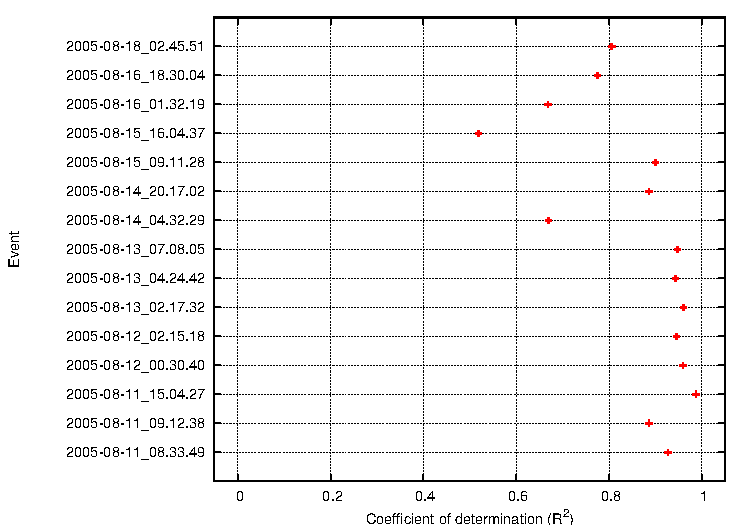
\includegraphics[width=\hsize]{./evaluation/figs/fidelity/seismicArrival/arrivalTimesPlotReg.pdf}
%% \end{center}
%% \caption{\small{\bf Coefficient of determination ($R^{2}$) for events.}
%% {\em The coefficien of determination is a measure of how well the
%% regression line represents the data.  A coefficient value greater than
%% 0.65 is generally described as a strong correlation.  As we can see,
%% most of our events have a coorelation higher than 0.65 indicating a good fit.}}
%% \label{fig-seismicArrivalReg}
%% \end{figure}


%% \begin{figure}[t]
%% \begin{center}
%% 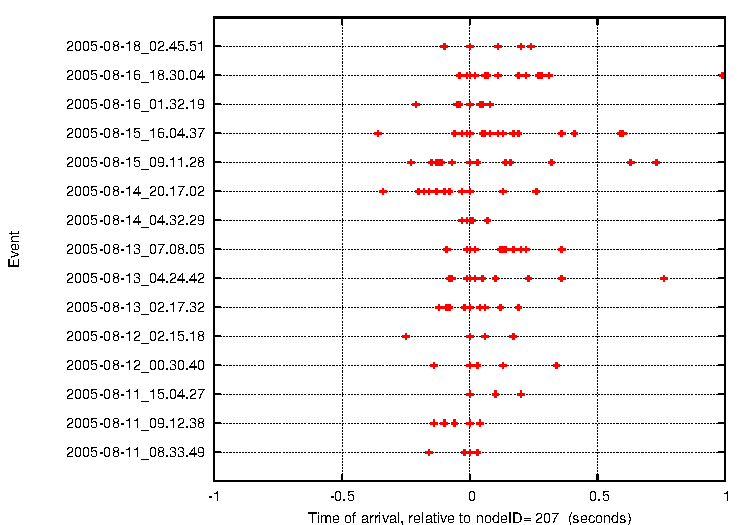
\includegraphics[width=\hsize]{./evaluation/figs/fidelity/seismicArrival/arrivalTimesPlotScatteredEvent.pdf}
%% \end{center}
%% \caption{\small{\bf Time of arrival of nodes for each event.}
%% {\em This graph shows the spread of arrival times.  The arrival times
%% are relative to node 207.  As we can see, most arrival times are
%% within a 1 second window of each other with a few outliers.}}
%% \label{fig-seismicArrivalScatteredEvents}
%% \end{figure}

%\begin{figure}[t]
%\begin{center}
%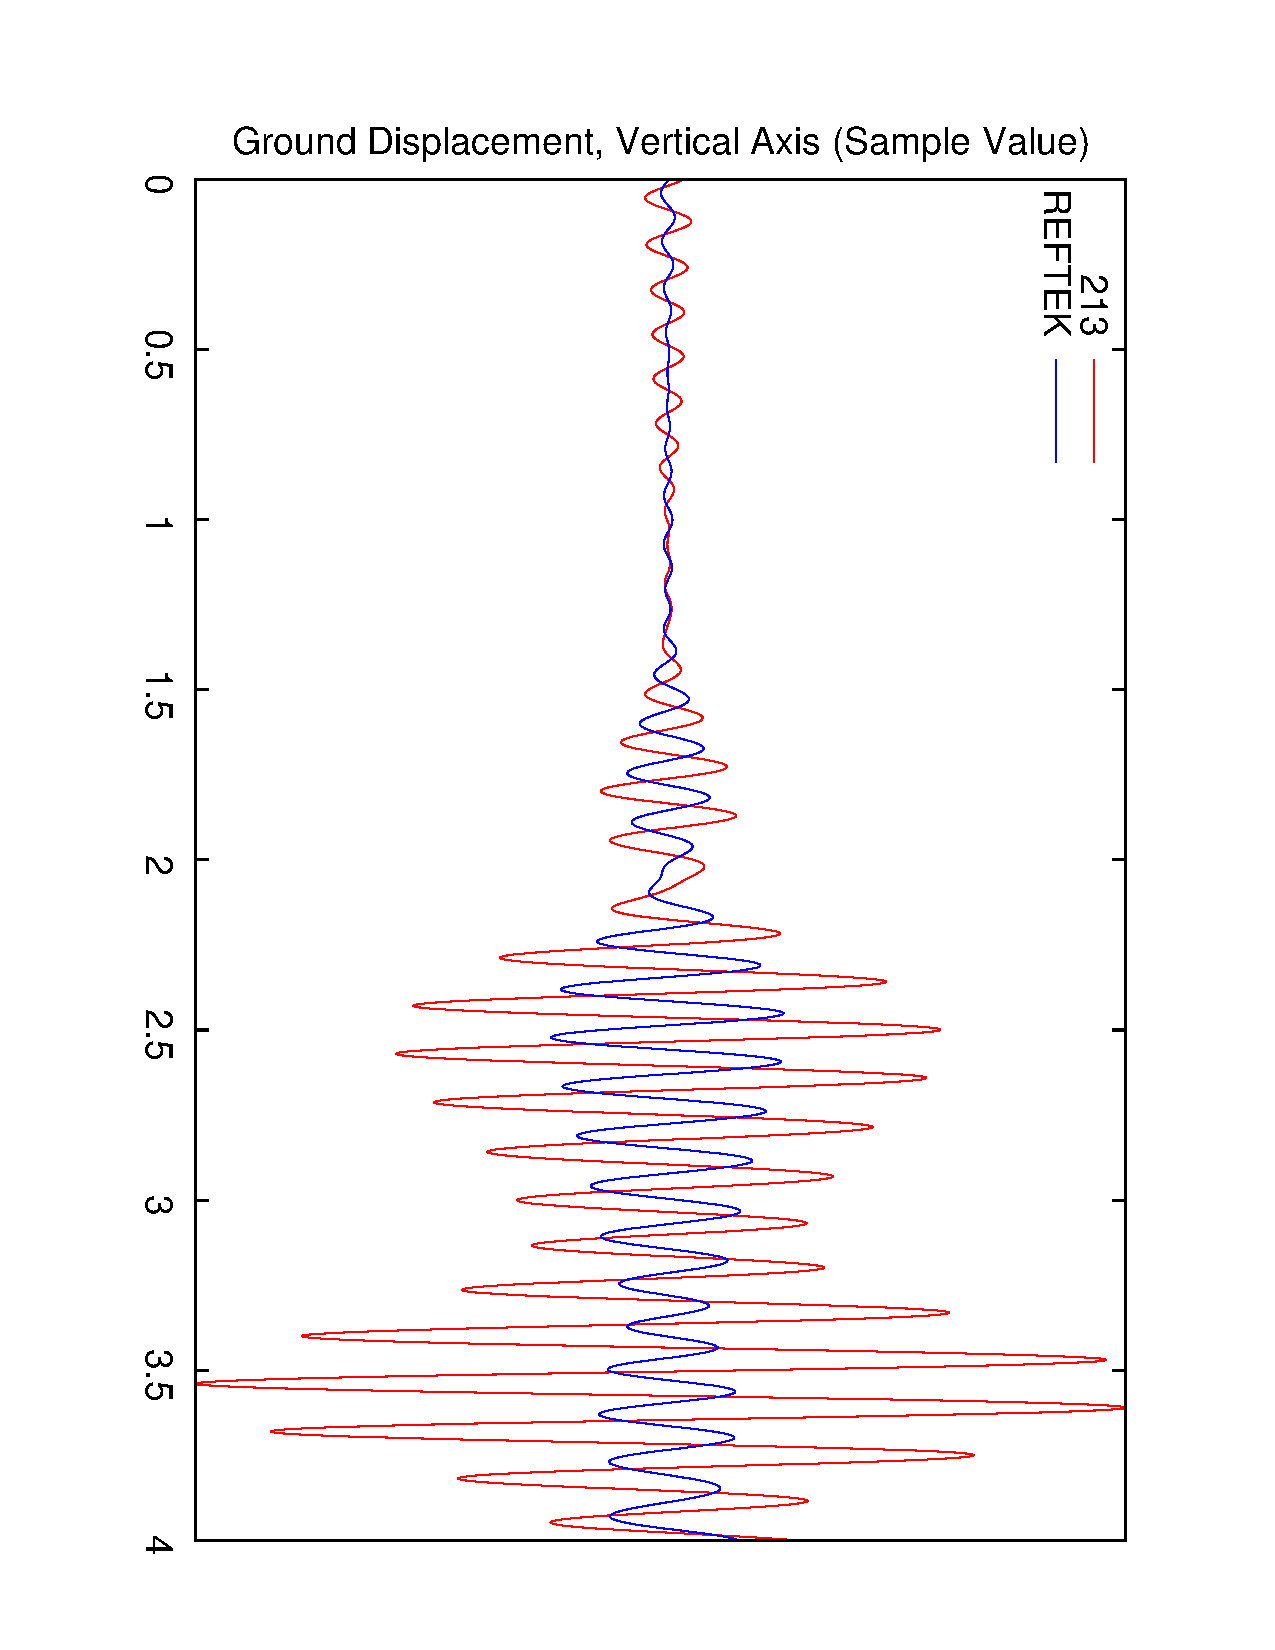
\includegraphics[width=0.8\hsize,angle=90]{./evaluation/figs/timing/ReftekV213/2005-08-15_16.04.37/213VREFTEK-NO-OFFSET.pdf}
%(a)
%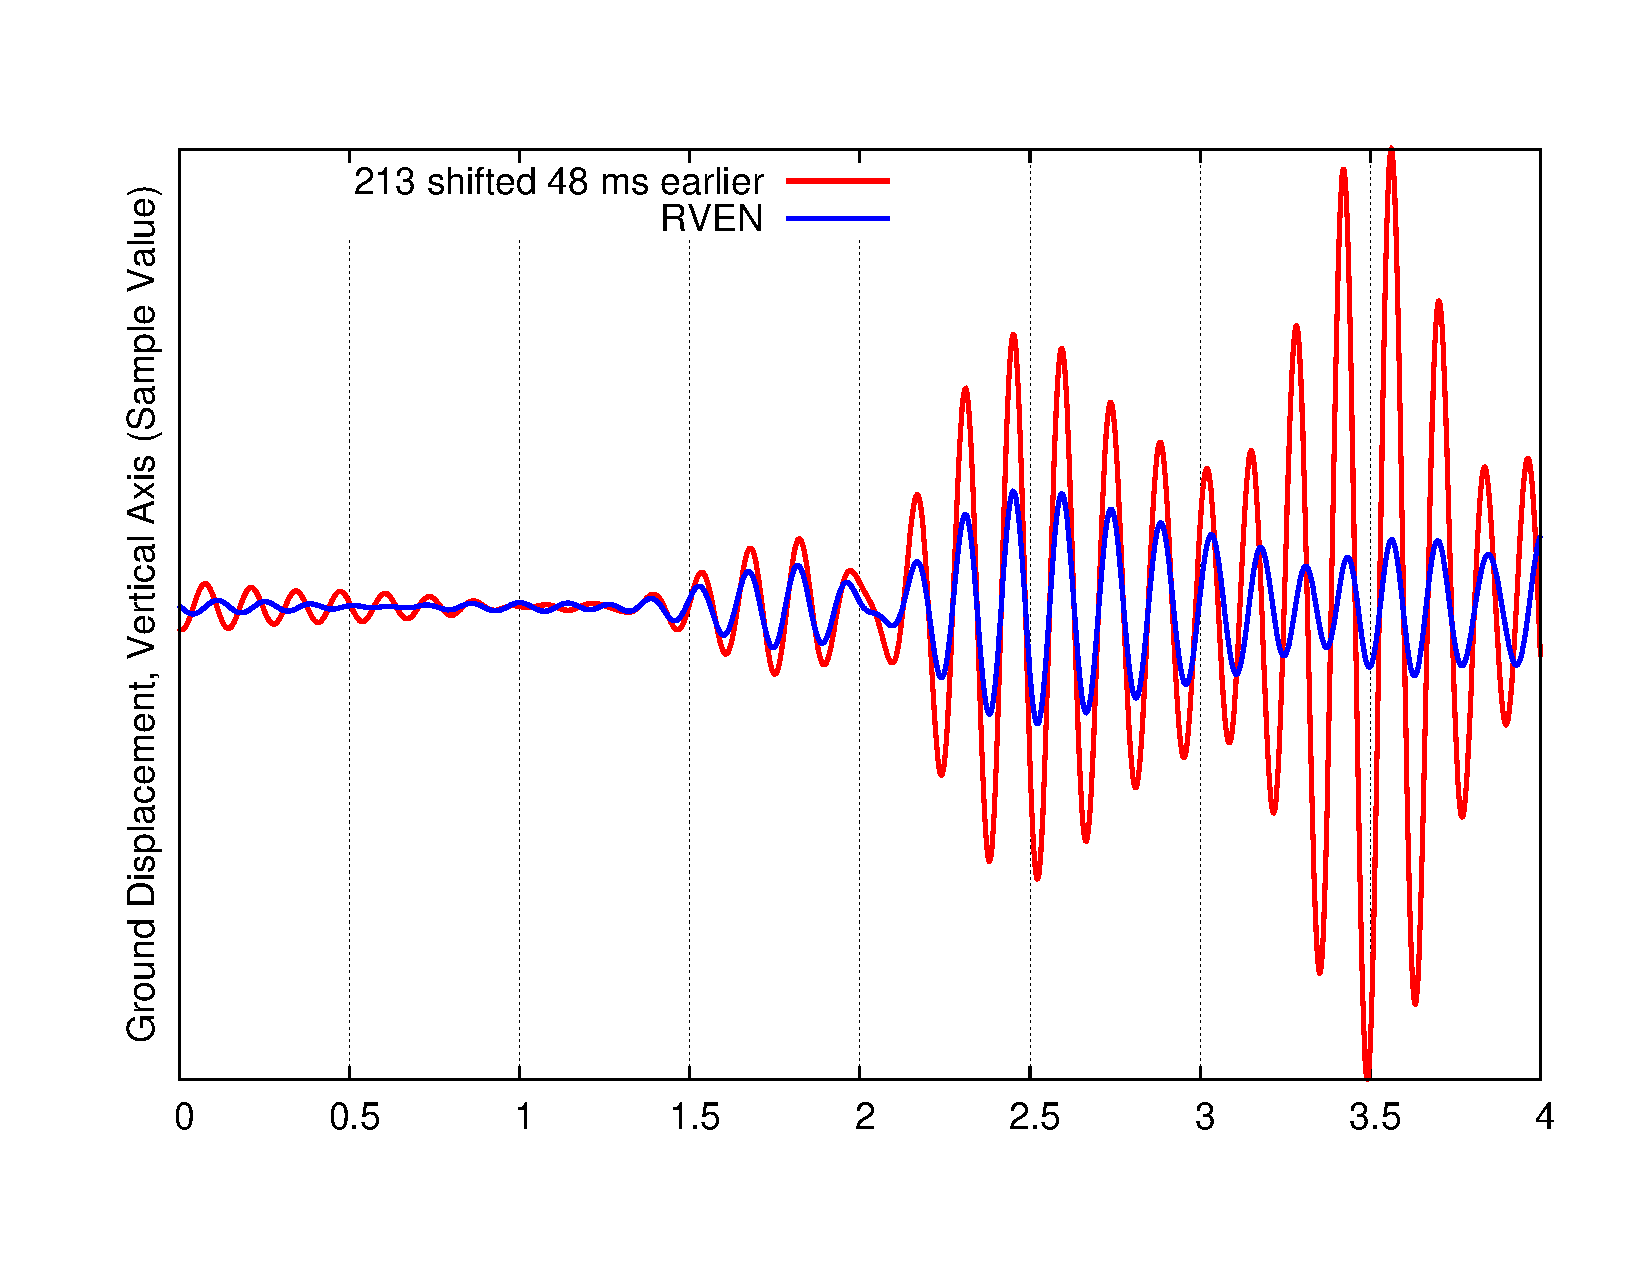
\includegraphics[width=0.8\hsize,angle=90]{./evaluation/figs/timing/ReftekV213/2005-08-15_16.04.37/213VREFTEK-POSITIVE48MS-OFFSET.pdf}
%(b)
%\end{center}
%\caption{\small{\bf Comparison of Node 213 and Reftek Signals}
%{\em The figures above show two signals, one collected by a sensor
%network station, Node 213, the other collected by a Reftek data logger
%attached to a broadband seismometer. Figure (a) shows the signals before a
%shift is applied, and Figure (b) shows the signals with a 48 ms shift
%applied. Both signals have been bandpass filtered between 6 and 8 Hz to
%reduce the differences in instrument response.  As these figures show a 48 ms
%shift produces a good match at the arrival time of the energy.  The
%signals are expected to differ throughout the coda showing the arrival of
%S-waves. \GWAnote{Need a better way to describe this...}}}
%\label{fig-rvenv213}
%\end{figure}

